\chapter{Instrukcja użytkownika}

\section{Graficzny interfejs użytkownika}

\label{gui}

Posługiwanie się przez użytkownika wszystkimi wymienionymi funkcjonalnościami powinno być łatwe oraz intuicyjne. Dostępne opcje zostały zaimplementowane w taki sposób, aby przeciętny odbiorca oprogramowania mógł dokonać żądanych działań w jak najkrótszym czasie i z jak najmniejszym wysiłkiem. Dostęp do większości funkcji uzyskiwany jest poprzez kliknięcia myszką komputera, która jest łatwiejszym sposobem nawigowania przez użytkowników wewnątrz aplikacji niż klawiatura.

Interakcja odbiorcy z aplikacją TeamSync poprzez klawiaturę została zredukowana do niezbędnego minimum, czyli wprowadzania danych (komentarzy, tytułów wątków, tożsamości oraz łańcucha \emph{secret} podczas dodawania nowego folderu itp.) oraz wyszukiwania fraz tekstowych. Nie ma możliwości, aby użytkownik nawigując wewnątrz systemu musiał ręcznie wpisywać np. nazwę innego użytkownika będącego w systemie, którego komentarze chciałby wyświetlić --- zamiast wprowadzania tych danych ręcznie, system wylistuje użytkowników pozostawiając tylko konieczność wyboru poprzez manipulację myszką.

\subsection*{Struktura graficzna aplikacji}

\begin{figure}[htb]
  \vspace{5pt}
  \begin{center}
    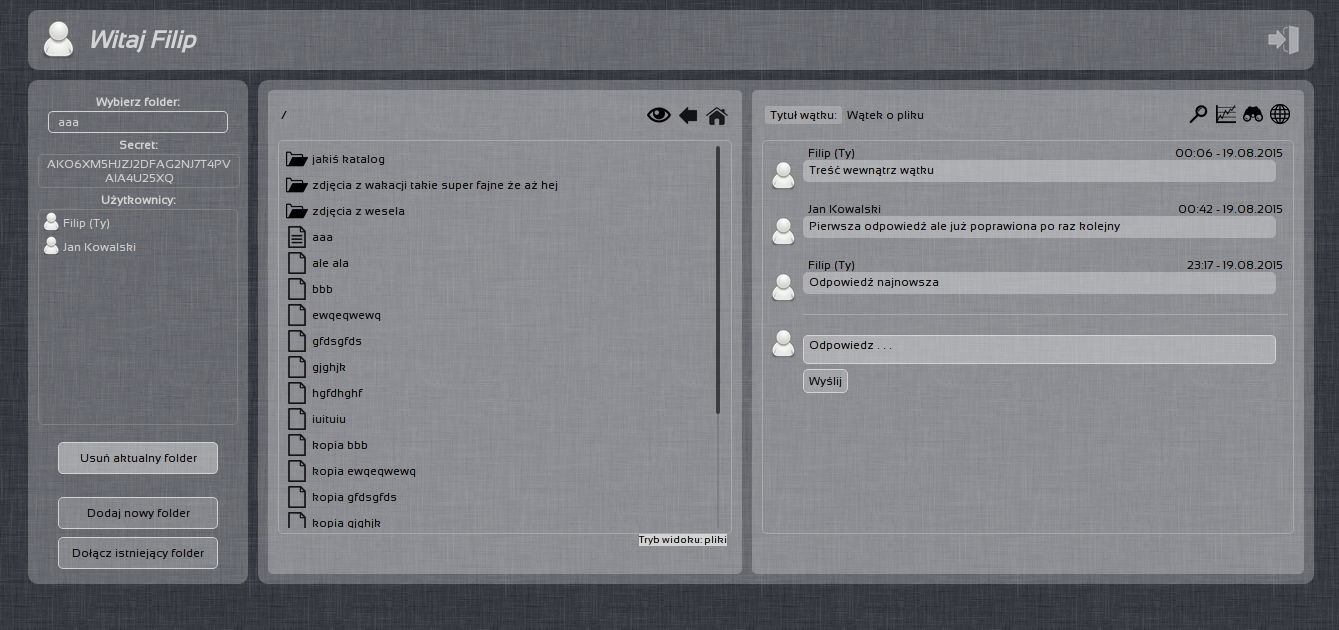
\includegraphics[width=400pt]{figures/filescomments.png}
  \end{center}
  \caption{Wygląd przykładowego folderu w graficznym interfejsie użytkownika.}
\end{figure}

Aby użytkownik łatwo odnalazł potrzebne mu funkcje ekran podzielony został na trzy części (nie licząc paska nagłówkowego) w układzie kolumnowym. Pierwsza --- część folderów --- służy do manipulacji synchronizowanymi katalogami. Druga --- środkowa --- służy do nawigacji po folderach oraz do przeglądania wątków, lecz nie wyświetlając wśród nich komentarzy. Trzecia natomiast przeznaczona jest do wyświetlania treści komentarzy i manipulowania zbiorem wyświetlanych wypowiedzi. Jeśli w danym momencie nie jest wybrany żaden z folderów z listy, dwie ostatnie części zajmujące główną część ekranu są nieaktywne.

W dalszej części podrozdziału omówione zostaną dokładniej przedstawione sekcje.

\subsubsection*{Sekcja folderów}

Jak opisano wcześniej, wewnątrz najmniejszej z trzech sekcji użytkownik może wykonywać operacje związane folderami, które współdzieli z innymi użytkownikami. Znajduje się w niej między innymi lista wszystkich zsynchronizowanych folderów (według ograniczeń systemu BitTorrent Sync może ich być maksymalnie $10$) wewnątrz kontrolki typu \emph{drop-down list} \cite{dropdownlist}, dzięki której użytkownik może w łatwy sposób dokonać wyboru.

Poniżej listy folderów znajdują się obszary, które po wybraniu katalogu wypełniają się odpowiednio danymi: ciągiem znaków tzw. \emph{secretem} oraz listą użytkowników, którzy przynależą do wybranego folderu. Aby ułatwić użytkownikowi identyfikację samego siebie spośród innych, do wyświetlanej nazwy jest dodawany ciąg znaków ,,(Ty)''.

Poza powyżej wymienionymi danymi w sekcji folderów znajdują się również przyciski umożliwiające usunięcie aktualnie wybranego folderu (przycisk jest nieaktywny, jeśli żaden folder nie został jeszcze wybrany) oraz dodanie nowego katalogu, które może odbyć się na dwa sposoby. Pierwszy zakłada, że folder jest inicjowany od zera i nie ma potrzeby wpisywania łańcucha \emph{secret}, ponieważ zostanie on wygenerowany przez system. Drugi wymaga jego podania i łączy wskazany z systemu plików pusty katalog z folderem innego użytkownika, od którego otrzymano łańcuch \emph{secret}. W obydwóch przypadkach konieczne jest podanie ścieżki do folderu, który ma być uwspólniony oraz tożsamości, czyli nazwy wyświetlanej dla innych użytkowników, mającej swój zasięg tylko wewnątrz katalogu.

\subsubsection*{Sekcja wątków}

Sekcja wątków składa się z nagłówka oraz części głównej zajmującej przeważający obszar całej sekcji. W nagłówku wyświetlana jest ścieżka aktualnej lokalizacji (nie bezpośrednia, lecz ta wewnątrz folderu, który będzie ,,korzeniem'' ścieżki), w której znajduje się użytkownik, zmieniająca się dynamicznie w interfejsie w miarę postępu nawigacji po katalogu.

Wewnątrz nagłówka, po przeciwnej stronie ścieżki znajdują się ikony funkcji, które pomagają w nawigacji oraz zmianie trybu widoku w głównej części sekcji. Naciśnięcie ikony prezentującej strzałkę skierowaną w lewo (,,do tyłu'') powoduje cofnięcie się ścieżki lokalizacji o jeden poziom. Uruchomienie funkcji ukrytej pod ikoną domu sprawia, że --- niezależnie od obecnej lokalizacji, w której się znajduje --- użytkownik zostanie sprowadzony do podstawowego poziomu w folderze --- jego ,,korzenia''.

Główna część sekcji służy do prezentacji plików oraz wątków w dwóch możliwych trybach, pomiędzy którymi przełączanie odbywa się za pomocą wciśnięcia kursorem myszki ikony zawierającej grafikę przedstawiającą oko, w nagłówku sekcji wątków.

\begin{description}[noitemsep]
  \item[Tryb plików] --- uruchamiając ten tryb, użytkownik może przeglądać zawartość synchronizowanego folderu w takiej postaci, w jakiej jest on zapisany na dysku. Uruchamiając kliknięciem myszy element z ikoną przedstawiającą folder użytkownik przechodzi do lokalizacji wewnątrz niego. Oprócz plików i katalogów wylistowanych w trybie plików, użytkownik widzi również wątki --- nie tylko te umieszczone w odpowiedniej lokalizacji ale też te przyporządkowane do konkretnych plików (jeśli do pliku jest przypisany wątek, ikona reprezentująca ten plik jest dostrzegalnie zmieniona, a po jej kliknięciu rozwijana jest lista wszystkich dyskusji dotyczących tego pliku).
  
  \item[Tryb wątków] --- przełączenie do tego trybu skutkuje wylistowaniem tylko i wyłącznie wątków napisanych wewnątrz folderu (niezależnie od lokalizacji), a uruchamianie funkcji nawigacji w tym trybie --- poprzez kliknięcia wewnątrz obszarów ikon (\emph{back} oraz \emph{home}) --- nie wywołuje żadnego efektu. Dodatkowo, wyświetlane są dwie ikony, dzięki którym użytkownik będzie miał możliwość posortować wątki według kilku kategorii oraz przefiltrować je według procentowego udziału grupy użytkowników wewnątrz nich (sekcja \ref{threadfiltering}). Obydwie te funkcje są dostępne z dodatkowych menu kontekstowych, pojawiających się w momencie kliknięcia kursorem myszki odpowiedniej ikony i umożliwiających precyzowanie dostępnych parametrów.
\end{description}


\subsubsection*{Sekcja komentarzy}

Sekcja komentarzy swoją strukturą oraz rozmiarami podobna jest do sekcji wątków --- zawiera nagłówek oraz część główną. Wewnątrz nagłówka znajduje się pole z opisem aktualnego widoku np. ,,Nowy wątek'', ,,Wątek:'' z tytułem aktualnej dyskusji lub ,,Wszystkie komentarze''. Obok wyświetlanego tekstu, wyrównane do prawej strony uszeregowane są ikony, za pomocą których możliwa jest manipulacja zbiorem, kolejnością lub filtracją pokazywanych komentarzy.

Poniżej znajduje się lista dostępnych ikon wraz z opisem uruchamianych przez nie funkcji.

\begin{description}[noitemsep]
  \item[Ikona zmiany widoków] --- prezentowana jako globus. Klikając na nią kursorem, użytkownik uaktywnia menu kontekstowe, które zawiera w sobie jedną kontrolkę typu \emph{drop-down list} z pięcioma wartościami: \emph{nowy wątek}, \emph{aktualny wątek}, \emph{wszystkie komentarze z lokalizacji}, \emph{wszystkie kometarze użytkownika}, \emph{wszystkie komentarze}. Jeśli użytkownik wybierze opcję \emph{wszystkie komentarze użytkownika}, wyświetlana jest dodatkowa kontrolka typu \emph{drop-down list} wewnątrz której wylistowani są użytkownicy. Dokładniejszy opis efektów użycia widoków znajduje sie w sekcji \ref{views}.
  
  \item[Ikona zmiany spójności] --- ikona przedstawiająca lornetkę, służy do uruchamiania menu kontekstowego zawierającego jedną kontrolkę typu \emph{drop-down list} zawierającą \texttt{n + 1} pozycji, gdzie \texttt{n} to liczba użytkowników współdzielących folder. Pierwsza wartość wyświetlana na liście to ,,NTP (globalna spójność)'', natomiast pozostałe elementy to nazwy użytkowników. Użyteczność tej funkcjonalności została dokładnie opisana w sekcji \ref{consistencies}.
  
  \item[Ikona statystyk] --- graficznie przedstawiona jako wykres. Za jej pomocą użytkownik może wyświetlić statystyki napisanych komentarzy w aktualnym ich zbiorze. Generowane zestawienie zawiera listę wszystkich autorów postów wraz z:
  \begin{itemize}[noitemsep]
    \item sumaryczną liczbą komentarzy użytkownika,
    \item łączną liczbą wszystkich komentarzy,
    \item procentowym udziałem postów użytkownika w aktualnym zbiorze wypowiedzi.
  \end{itemize}
  Użytkownik może niezależnie od widoku w jakim obecnie pracuje przejść poprzez kliknięcie kursorem myszy w ikonę statystyk do trybu, w którym wyświetlane jest wyłącznie zestawienie z wymienionymi wyżej danymi. Aby z powrotem móc czytać komentarze, należy ponownie kliknąć ikonę. Statystyki zawsze będą obejmowały zakres aktualnego widoku --- jeśli użytkownik przegląda konkretny wątek, zestawienie zostanie wygenerowane tylko dla tego wątku.
  
  \item[Ikona wyszukiwania] --- reprezentowana przez grafikę przedstawiającą lupę. Jej naciśnięcie powoduje pojawienie się wewnątrz nagłówka, tuż obok ikony pola tekstowego, do którego użytkownik musi wpisać wyszukiwaną frazę. W trakcie wpisywania szukanego tekstu komentarze są przeszukiwane i odfiltrowane są te z nich, które nie pasują do wpisanego przez użytkownika wzorca. Po ponownym wciśnięciu ikony, interfejs graficzny usuwa pole tekstowe z ekranu, a odrzucone wcześniej komentarze zostają przywrócone. Dzieje się tak z uwagi na fakt, że filtr wyszukiwania działa tylko w momencie, gdy pole tekstowe, do którego należy wpisać szukaną frazę, jest widoczne.
\end{description}

Ikony będące wewnątrz nagłówka są dynamicznymi elementami interfejsu graficznego --- jeśli nie są potrzebne, nie są wyświetlane. Ma to miejsce np. podczas zamieszczania nowego wątku --- podczas wpisywania jego tytułu oraz treści pierwszego komentarza nie ma potrzeby wyszukiwania czegokolwiek w komentarzach, ani zmiany spójności kolejności wypowiedzi w wątku. Podobnie, jeśli żaden z wątków nie został jeszcze wybrany --- a więc komentarze nie są jeszcze wyświetlane --- to ikony spójności, statystyk oraz wyszukiwania nie są potrzebne użytkownikowi. Nie są więc wyświetlane w interfejsie, co wpływa na jego przejrzystość oraz awaryjność (uniemożliwianie popełniania błędów przez użytkownika).

W części głównej sekcji komentarzy znajdują się wypowiedzi użytkowników wewnątrz dodających przejrzystości ramek, otoczone dodatkowymi danymi takimi jak:

\begin{itemize}[noitemsep]
  \item grafika przedstawiająca tzw. ,,avatar'' użytkownika,
  
  \item nazwa autora komentarza,
  
  \item czas i data umieszczenia komentarza w formacie pobranym z pliku konfiguracyjnego (sekcja \ref{configteamsync}),
  
  \item jeśli zbiór komentarzy obejmuje więcej niż jeden wątek, dodatkowo blisko pod wypowiedzią zamieszczany jest tytuł dyskusji, z której pochodzi komentarz. Jest on hiperłączem prowadzącym do całej zawartości wątku, z którego pochodzi wypowiedź, dzięki czemu użytkownik poprzez jedno kliknięcie myszy może przejśc do całej rozmowy i łatwo zapoznać się z kontekstem, w którym został umieszczony interesujący go komentarz.
\end{itemize}

Graficzny interfejs aplikacji TeamSync w łatwy sposób umożliwia edycję komentarzy oraz przeglądanie historii zmian każdej z wypowiedzi (o ile taka zmiana miała miejsce). Jeśli użytkownik jest autorem komentarza, po umieszczeniu nad nim kursora w sekcji komentarzy wyświetlona zostanie dodatkowa ikona przedstawiająca długopis obok treści wypowiedzi. Po jej uruchomieniu cała aktualna treść komentarza zostanie umieszczona wewnątrz pola tekstowego i dodane zostaną dodatkowe dwa przyciski pod polem tekstowym: przycisk zatwierdzający zmianę treści oraz anulujący ją.

Umieszczenie kursora myszki nad przynajmniej raz zmodyfikowanym przez autora komentarzem skutkuje pojawieniem się --- w miejscu tuż obok ikony edycji wypowiedzi --- ikony historii posta. Po jej uruchomieniu zostaje wyświetlona lista z wcześniejszymi wersjami komentarza wraz z czasem i datą zmiany jego treści.

Użytkownik przeglądający komentarze w obrębie jednego wątku ma możliwość szybkiego zabrania głosu w dyskusji --- za ostatnim, najnowszym komentarzem znajduje się pole tekstowe, do którego wpisywana jest treść odpowiedzi oraz przycisk zatwierdzający komentarz. Po zatwierdzeniu, wprowadzona wypowiedź będzie wypowiedzią najświeższą i system gotowy jest do dalszej pracy.

\section{Widoki}

\label{views}

Aby stworzyć użytkownikowi jak najlepsze warunki do łatwego i szybkiego przeglądania komentarzy, wyszukiwania zawartych w nich informacji lub przeglądania statystyk ich dotyczących zaimplementowano tzw. ,,widoki'', pomiędzy którymi użytkownik może wybierać w zależności od aktualnej potrzeby. Jako widok można rozumieć zakres komentarzy wyświetlanych w aplikacji. Użytkownik ma do wyboru pięć widoków, między którymi może w dowolnej chwili wybrać, jednak nie pomiędzy wszystkimi widokami jest możliwe przejście. Dodatkowo, w niektórych przypadkach przejść międyz widokami jest możliwość utraty części danych np. niezatwierdzoną odpowiedź w którymś z wątków.

\subsection*{Widok nowego wątku}

Widok, który uruchamiany jest podczas inicjowania wątku. Nie są wyświetlane w nim żadne komentarze, a użytkownik proszony jest o podanie tytułu wątku, treści pierwszego komentarza oraz ewentualnego pliku, którego wątek będzie dotyczył. Do trybu nowego wątku można przejść wyłącznie poprzez wciśnięcie przycisku ,,Nowy wątek'' w jednej z lokalizacji, bądź ,,Nowy wątek w pliku'', jeśli dyskusja będzie dotyczyć pliku (użytkownik musi wskazać konkretny plik z sekcji plików). Taka forma rozpoczęcia wątku jest konieczna ze względu na konieczność wskazania aplikacji lokalizacji wątku. Opcja ,,Nowy wątek'' wewnątrz rozwijanego menu w interfejsie graficznym --- dotyczącego zmiany widoku --- jest zablokowana.

\subsection*{Widok aktualnego wątku}

Widok uruchamiany, gdy użytkownik wybierze z listy plików element z ikoną wątku lub dowolny element z listy wątków. Po wybraniu dyskusji następuje odczytywanie komentarzy z folderu z wątkiem przez serwer i wyświetlenie ich przez przeglądarkę w graficznym interfejsie. Przejście do tego widoku jest możliwe wyłącznie poprzez uruchomienie kursorem odpowiedniego elementu z listy plików lub wątków. Aplikacja musi otrzymać precyzyjną informację, którą konkretnie dyskusję użytkownik chce przeczytać, aby ją wyświetlić. Podobnie jak w przypadku widoku nowego wątku, opcja w menu ,,Aktualny wątek'' jest zablokowana podczas przeglądania komentarzy w innym widoku.
  
\subsection*{Widok z bieżącej lokalizacji}
  
Zakres komentarzy w tym widoku obejmuje wypowiedzi z wszystkich dyskusji pobranych z bieżącej lokalizacji --- tej, którą użytkownik obecnie przegląda w przeglądarce plików. Przejście do tego widoku możliwe jest z każdego innego widoku, użytkownik musi jednak liczyć się z możliwą utratą treści np. podczas tworzenia nowego wątku lub odpowiedzi w już istniejącym. Podczas przełączania widoków wpisywane i niezatwierdzone dane w tych polach tekstowych są tracone.

\subsection*{Widok wszystkich komentarzy użytkownika}

Aplikacja wyświetli wyłącznie te wypowiedzi, których autorem jest wybrany użytkownik. Podobnie jak z widokiem dotyczącym lokalizacji, przejście na niego jest możliwe w każdym momencie i należy liczyć się z możliwością utraty danych.

\subsection*{Widok wszystkich komentarzy}

Zakres wyświetlanych komentarzy obejmujący wszystkie komentarze wprowadzone do aplikacji niezależnie od ich lokalizacji lub autora. Do tego widoku użytkownik może przejść w dowolnym momencie licząc się z utratą niezatwierdzonych komentarzy lub wątków. Przydatny użytkownikowi, gdy chce wyszukać ciąg tekstowy w bazie wszystkich wypowiedzi.

\section{Filtrowanie listy wątków}

\label{threadfiltering}

Celem aplikacji TeamSync jest nie tylko zaawansowana manipulacja umieszczanymi komentarzami, ale również możliwość łatwego wyszukiwania dyskusji na poziomie nie pojedynczych wypowiedzi, a całych wątków. Jeśli użytkownik chciałby wydzielić z wszytkich dyskusji takie, w których wybrani przez niego użytkownicy brali większościowy bądź mniejszościowy udział, system umożliwi mu to za pomocą intuicyjnego menu kontekstowego uruchamianego w sekcji plików ikoną przedstawiającą grupę ludzi.

Uruchamiając tą część interfejsu użytkownik ma możliwość zaznaczyć użytkownika (jednego lub kilku) z listy wszystkich użytkowników współdzielących folder i wybrać próg procentowy dla zaangażowania wybranych użytkowników w wątek. Dostępne progi procentowe to \texttt{10\%}, \texttt{30\%}, \texttt{50\%}, \texttt{70\%}, \texttt{90\%}. Dodatkowo istnieje możliwość określenia, czy aplikacja ma wybrać te wątki, w których suma komentarzy wybranej grupy użytkowników jest większa od łącznej liczby wypowiedzi w wątku, czy te, w których jest ona mniejsza.

Przykładem użycia funkcjonalności mogłaby być sytuacja, w której użytkownik chciałby odnaleźć wątek nie pamiętając konkretnych treści komentarzy zawartych wewnątrz niego, natomiast pamiętając, że ilość wypowiedzi dwóch innych użytkowników (\texttt{A} oraz \texttt{B}) zdecydowanie zdominowała dyskusję, co rzadko ma miejsce w pozostałych wątkach. Wówczas --- ustawiając filtr według określonych preferencji (zaznaczony próg \texttt{\textgreater 70\%} lub \texttt{\textgreater 90\%} oraz wybrani użytkownicy \texttt{A} oraz \texttt{B} z listy wszystkich użytkowników) --- przy niewielkim wysiłku znacznie zawęziłby obszar poszukiwań wątku.

\section{Użycie wybranych funkcji interfejsu graficznego}

W niniejszej części dodatku zostaną zaprezentowane sposoby użycia wybranych funkcji systemu \emph{TeamSync}.

\subsection*{Tworzenie nowego wątku}

\begin{figure}[h!]
  \vspace{5pt}
  \begin{center}
    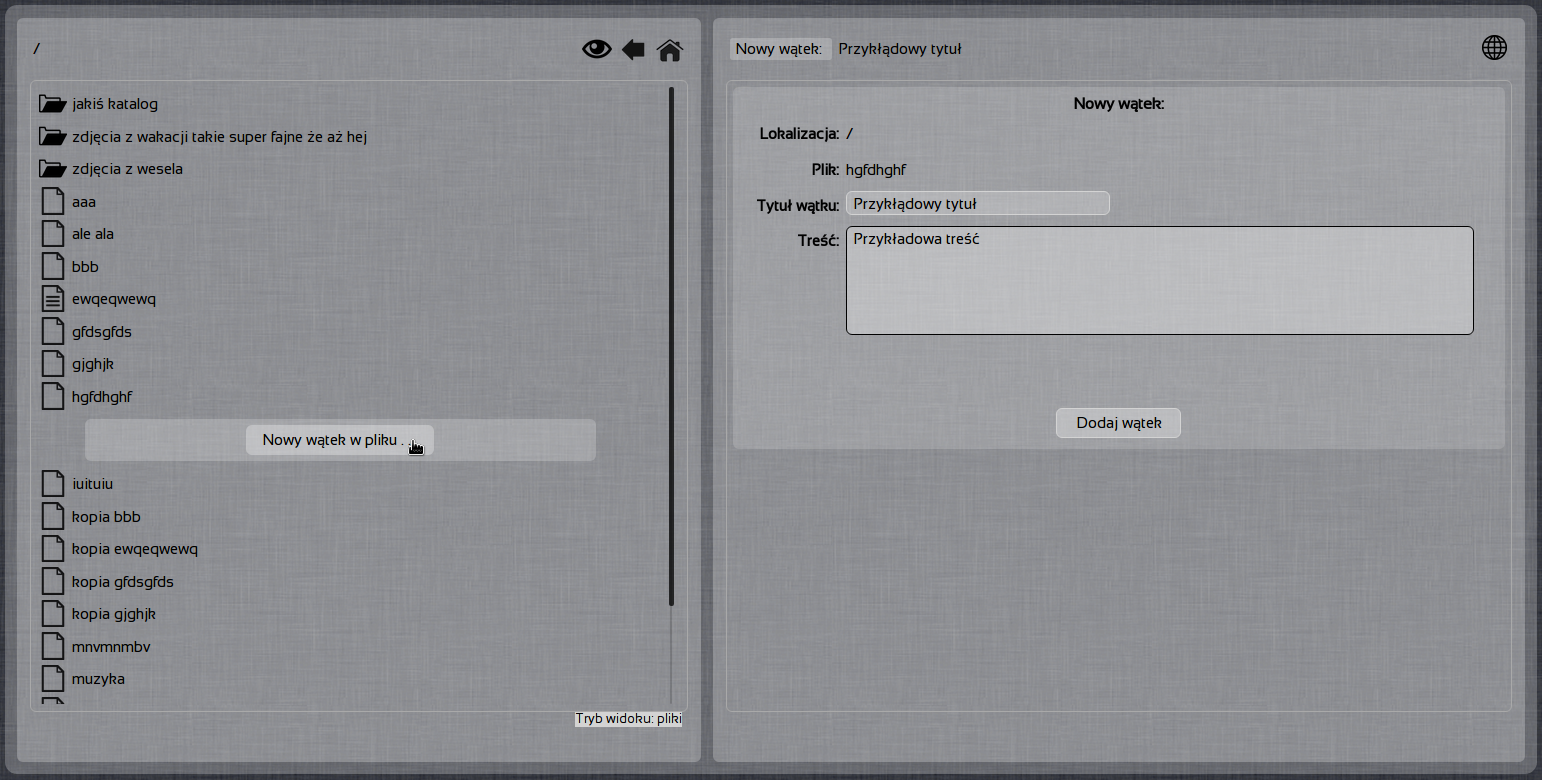
\includegraphics[width=400pt]{figures/screenshotnewthread1.png}
  \end{center}
  \caption{Zrzut ekranu z interfejsu graficznego podczas tworzenia nowego wątku.}
\end{figure}

Aby utworzyć nowy wątek w systemie, należy wykonać następujące kroki w sekcji plików:

\begin{enumerate}[noitemsep]
  \item Nawigując wewnątrz sekcji plików, znaleźć żądaną lokalizację wątku (lub żądany plik, któłrego ma dotyczyć dyskusja).
  
  \item Kliknąć kursorem myszy przycisk ,,\emph{Nowy wątek}'' (lub ,,\emph{Nowy wątek w pliku}'').
\end{enumerate}

Po wykonaniu powyższych czynności, następne kroki należy wykonać wewnątrz sekcji komentarzy, gdzie pojawią się puste pola tekstowe: ,,\emph{Tytuł wątku}'' oraz ,,\emph{Treść komentarza}'':

\begin{enumerate}[noitemsep]
  \item Uzupełnić wyżej wymienione pola tekstowe (w przypadku nie wypełnienia, zostanie wyświetlony odpowiedni komunikat).
  
  \item Zatwierdzić utworzenie nowego wątku przyciskiem ,,\emph{Dodaj wątek}''
\end{enumerate}

\subsection*{Wprowadzanie nowego komentarza}

\begin{figure}[h!]
  \vspace{5pt}
  \begin{center}
    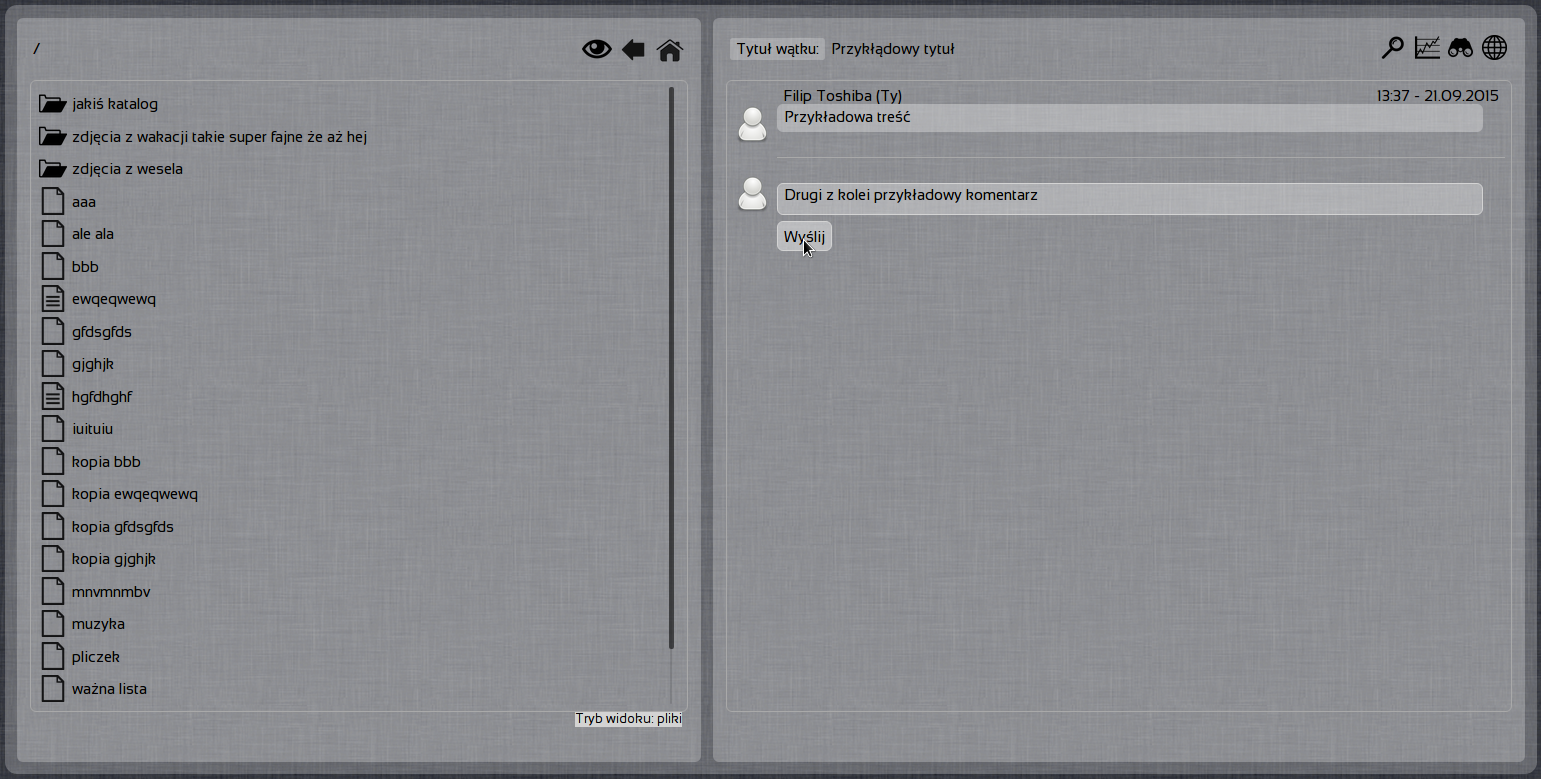
\includegraphics[width=400pt]{figures/screenshotnewcomment1.png}
  \end{center}
  \caption{Zrzut ekranu z interfejsu graficznego podczas dodawania nowego komentarza.}
\end{figure}

Podczas dodawania nowego komentarza użytkownik musi brać pod uwagę ograniczenie systemu polegające na tym, że aby umieścić nową wypowiedź, użytkownik powinien się znajdować w widoku aktualnego wątku (dokładny opis widoków znajduje się w sekcji \ref{views}). Jest to konieczne ze względu na fakt, iż nie będąc w widoku wątku, system nie będzie mógł umieścić komentarza w systemie plików, ponieważ nie będzie wiedział, w którym wątku stworzyć plik z nowym komentarzem.

Aby dodać nowy komentarz w dyskusji, użytkownik musi wykonać nastepujące kroki:

\begin{enumerate}[noitemsep]
  \item Po wyświetleniu komnetarzy z jednej dyskusji, użytkownik powinien przejść na sam dół sekcji komentarzy (tam, gdzie znajduje się najświeższa wypowiedź).
  
  \item Kliknięciem kursora myszy aktywować pole tekstowe i wpisać do niego treść wypowiedzi.
  
  \item Zatwierdzić komentarz przyciskiem ,,\emph{Dodaj}''.
\end{enumerate}

\subsection*{Modyfikacja komentarza}

\begin{figure}[h!]
  \vspace{5pt}
  \begin{center}
    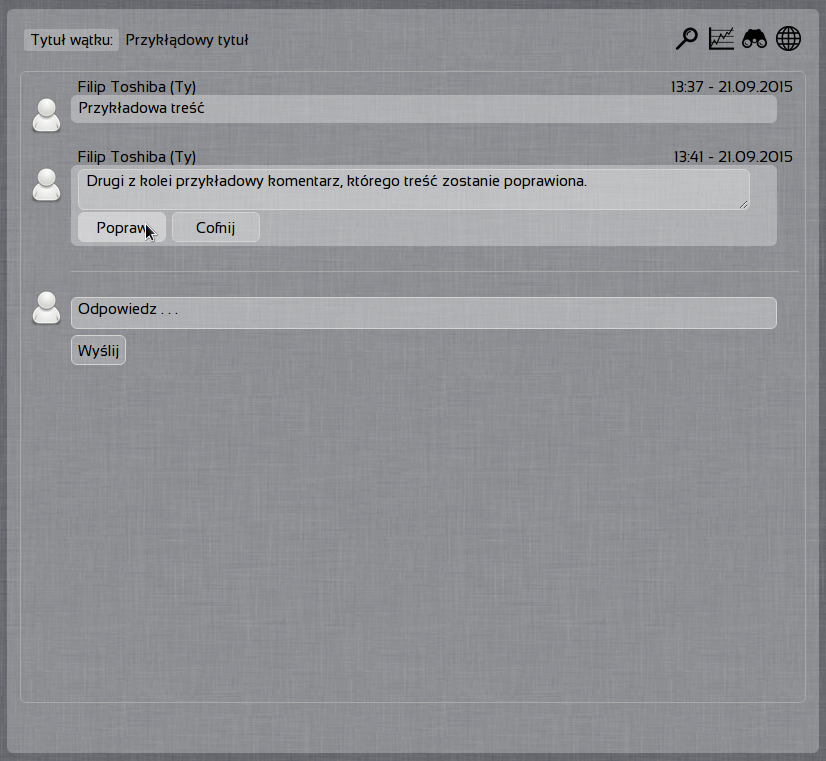
\includegraphics[width=240pt]{figures/screenshoteditcomment1.png}
  \end{center}
  \caption{Zrzut ekranu z interfejsu graficznego podczas edycji komentarza.}
\end{figure}

Jeśli użytkownik chce zmodyfikować treść komentarza, może tego dokonać, o ile jest jego autorem. Edycja treści odbywa się w sekcji komentarzy i przebiega w następujący sposób:

\begin{enumerate}[noitemsep]
  \item Po ustawieniu przez użytkownika kursora nad obszar komentarza wyświetlane są na nim przyciski inicjujące edycję oraz pokazujące historię zmian w jego treści (o ile zmiany kiedykolwiek nastąpiły).
  
  \item Po kliknięciu przycisku uruchamiającego edycję aktualny tekst komentarza umieszczany jest wewnątrz pola tekstowego, dodatkowo pojawia się przycisk akceptujący zmiany. Tekst jest edytowalny.
  
  \item Po wprowadzeniu zmian i zatwierdzeniu ich przyciskiem plik zk omentarzem jest modyfikowany.
\end{enumerate}

\newpage

\subsection*{Wyświetlanie historii zmian komentarza}

\begin{figure}[h!]
  \vspace{5pt}
  \begin{center}
    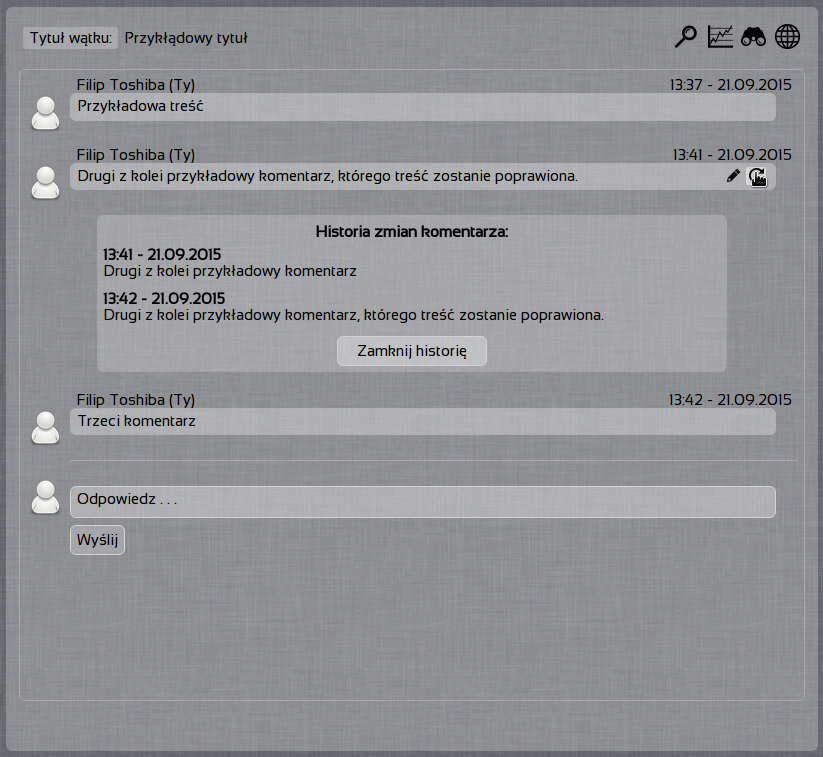
\includegraphics[width=240pt]{figures/screenshotcommenthistory1.png}
  \end{center}
  \caption{Zrzut ekranu z interfejsu graficznego podczas wyświetlania historii komentarza.}
\end{figure}

Przeglądanie historii zmian komentarzy jest możliwe tylko dla tych wypowiedzi, które zostały w przeszłości zmodyfikowane przez ich autorów. Historia może być wyświetlana przez każdego użytkownika w systemie. Przeglądanie modyfikacji odbywa się w sekcji komentarzy w następujący sposób:

\begin{enumerate}[noitemsep]
  \item Po ustawieniu przez użytkownika kursora nad obszar komentarza wyświetlane są na nim przyciski inicjujące edycję oraz pokazujące historię zmian w jego treści (o ile zmiany kiedykolwiek nastąpiły).
  
  \item Po uruchomieniu przycisku historii wyświetlona zostanie ramka pod komentarzem, zawierająca pełną treść komentarza po edycji, wraz z jej datą.
  
  \item Aby wyłączyć przeglądanie historii komentarza, należy kliknąć kursorem myszy na przycisk ,,\emph{Zamknij historię}'' wewnątrz ramki.
\end{enumerate}